\begin{frame}

    \centering
    \Huge{¿Que aplicaciones libres vienen preinstaladas?}

\end{frame}

\begin{frame}

    \frametitle{Aplicaciones libres preinstaladas}

    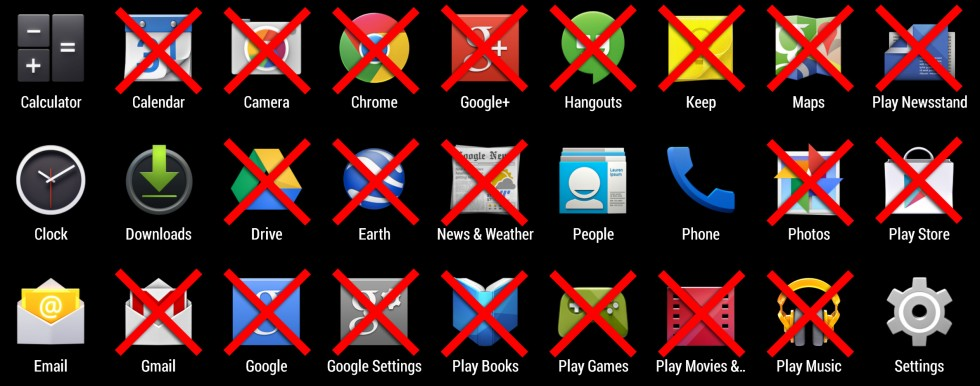
\includegraphics[width=\textwidth]{images/android-free-apps.jpg}

\end{frame}

\begin{frame}

    \frametitle{Alternativas libres a las aplicaciones más usadas}

    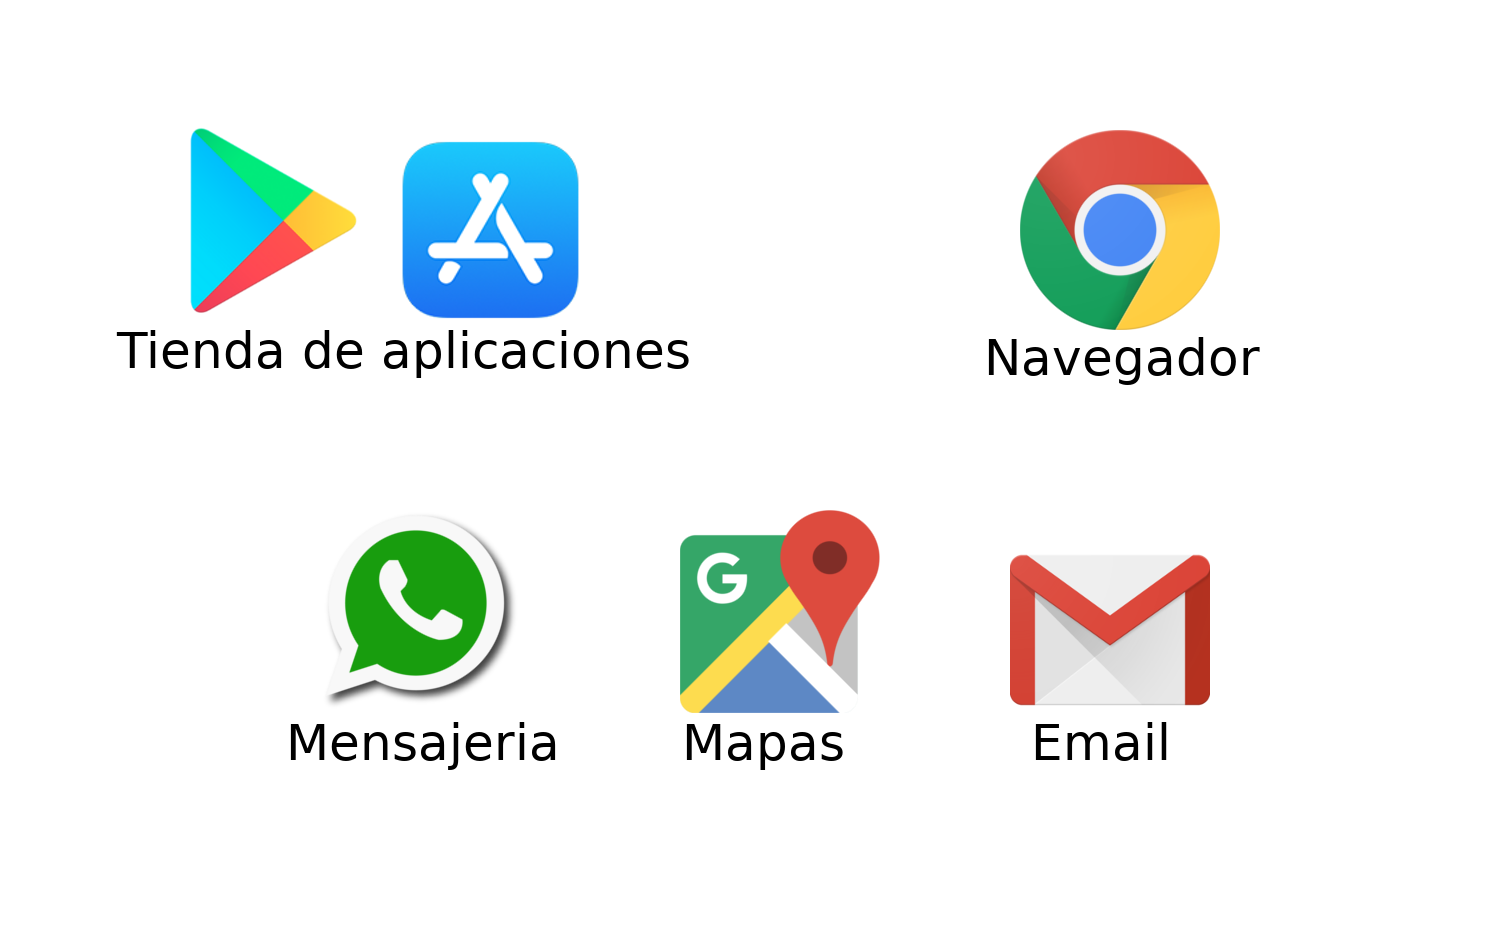
\includegraphics[width=\textwidth]{images/alternatives-title.png}

\end{frame}

\begin{frame}

    \frametitle{Tienda de aplicaciones - Aptoide}

    \begin{columns}[c]
        \column{.3\textwidth}
            \begin{center}
                
\includegraphics[height=0.15\textheight]{images/aptoide-logo.png}
                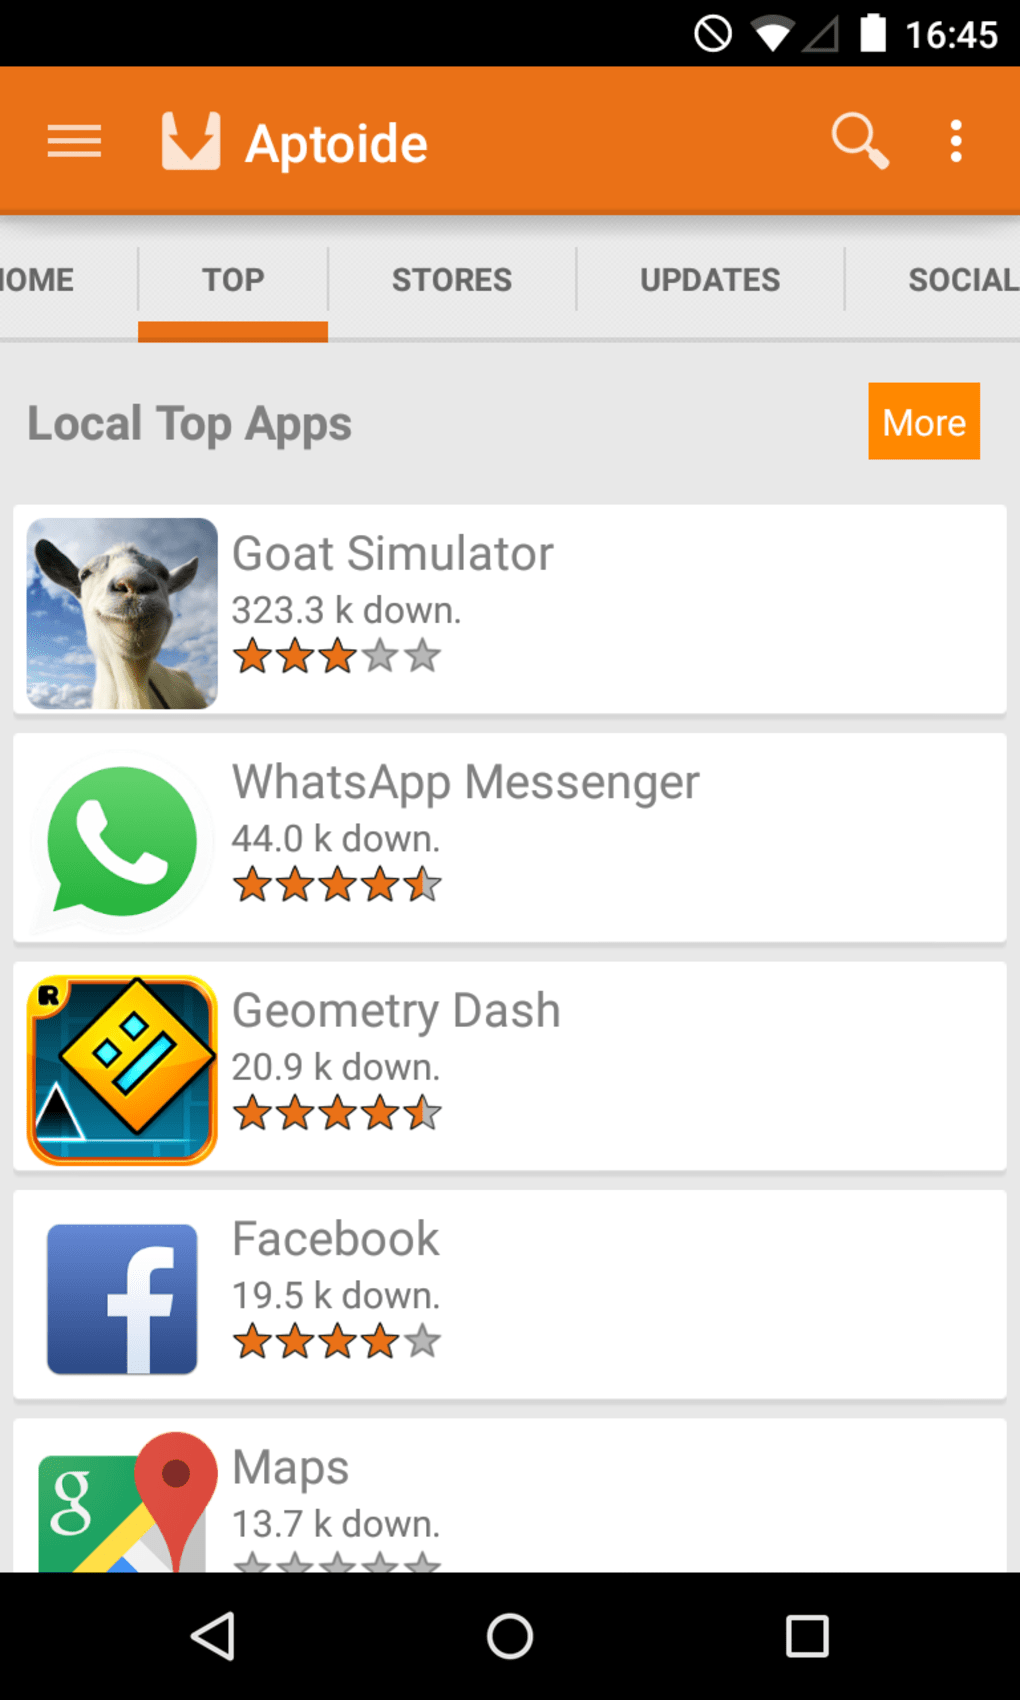
\includegraphics[height=0.5\textheight]{images/aptoide-screencap.png}
            \end{center}
        \column{.7\textwidth}
            \begin{itemize}
                \item Plataformas soportadas: Android
                \item Disponibilidad: \href{https://es.aptoide.com/}{Página web}
                \item Licencia: GPLv2
            \end{itemize}
    \end{columns}

\end{frame}

\begin{frame}

    \frametitle{Tienda de aplicaciones - F-Droid}

    \begin{columns}[c]
        \column{.3\textwidth}
            \begin{center}
                
\includegraphics[height=0.15\textheight]{images/fdroid-logo.png}
                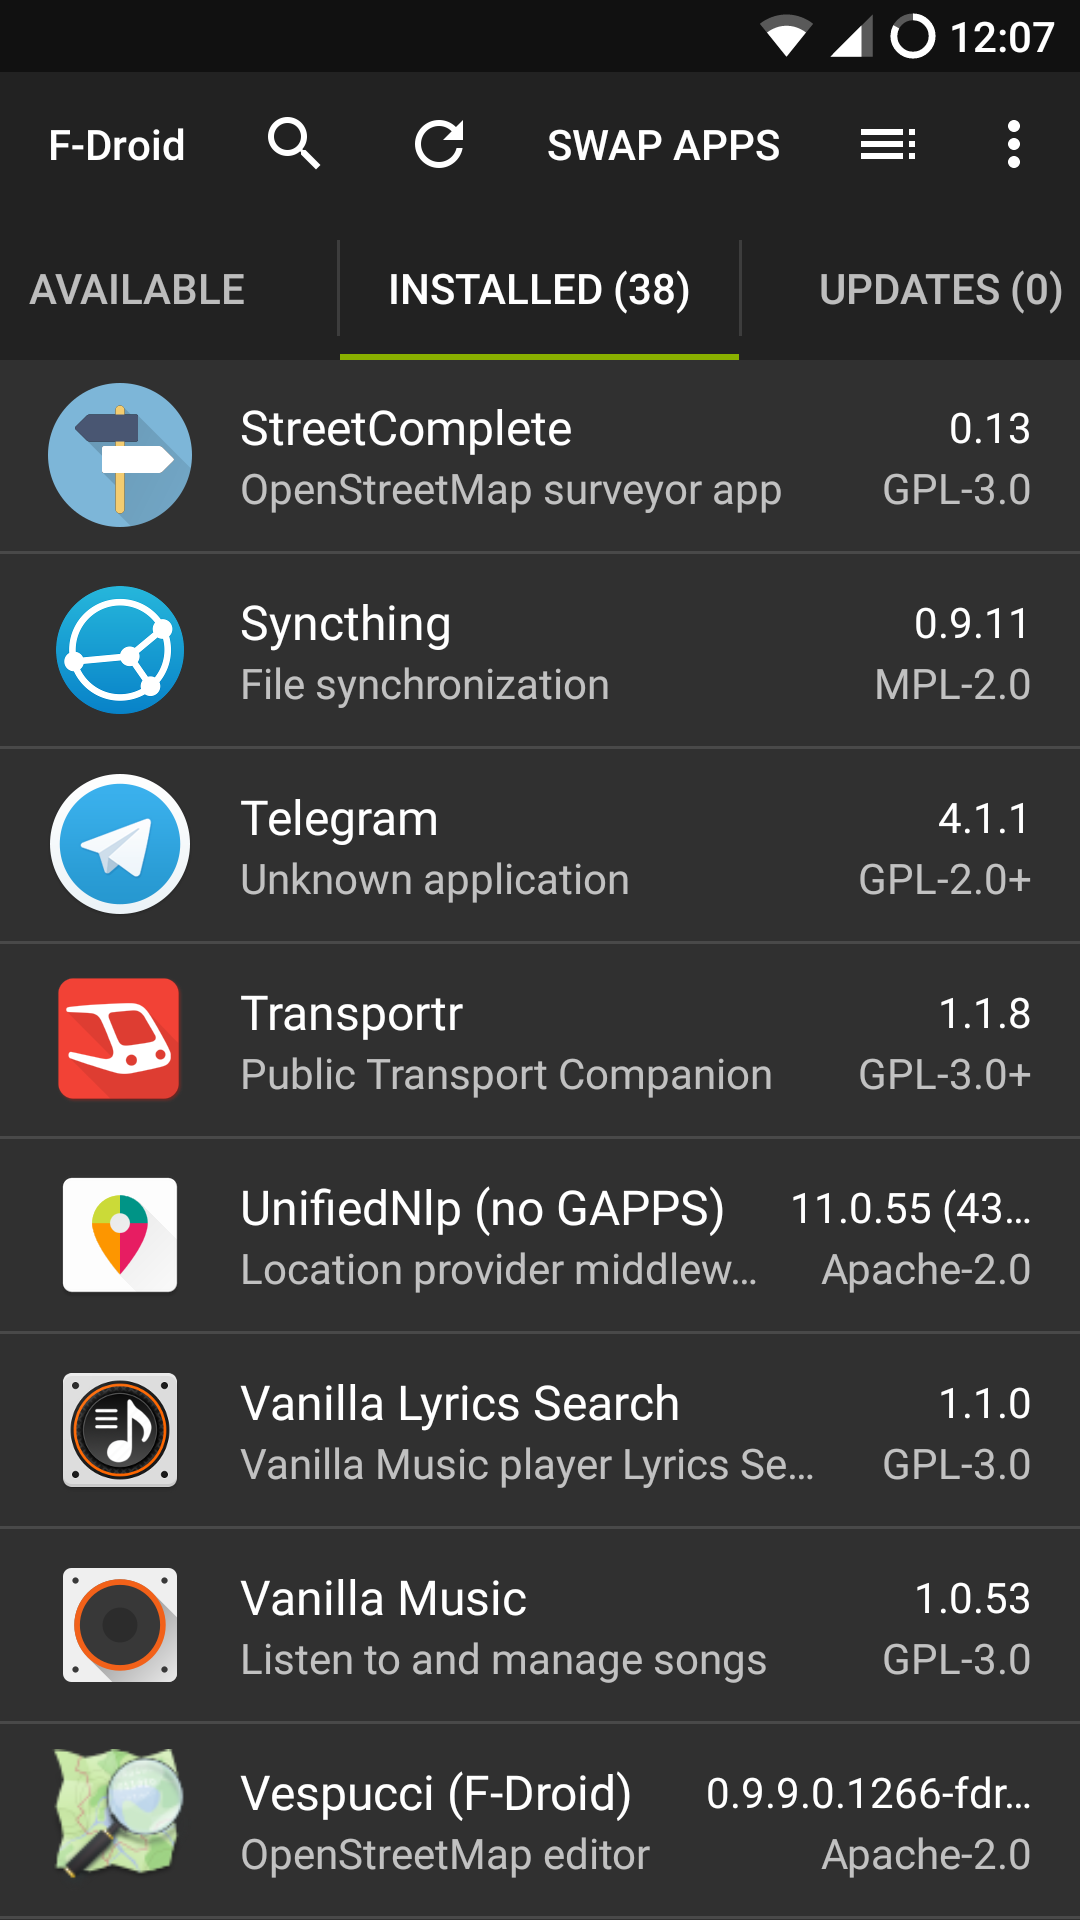
\includegraphics[height=0.5\textheight]{images/fdroid-screencap.png}
            \end{center}
        \column{.7\textwidth}
            \begin{itemize}
                \item Plataformas soportadas: Android
                \item Disponibilidad: \href{https://f-droid.org/es/}{Página web}
                \item Licencia: GPLv3
            \end{itemize}
    \end{columns}

\end{frame}

\begin{frame}

    \frametitle{Navegador - Firefox}

    \begin{columns}[c]
        \column{.3\textwidth}
            \begin{center}
                
\includegraphics[height=0.15\textheight]{images/firefox.png}
                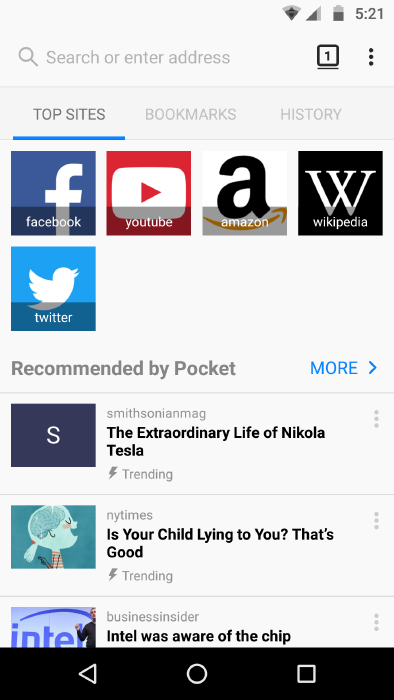
\includegraphics[height=0.5\textheight]{images/firefox-screencap.png}
            \end{center}
        \column{.7\textwidth}
            \begin{itemize}
                \item Plataformas soportadas: Android, iOS
                \item Disponibilidad: Play Store, App Store, F-Droid
                \item Licencia: MPL 2.0
            \end{itemize}
    \end{columns}

\end{frame}

\begin{frame}

    \frametitle{Navegador - Chromium}

    \begin{columns}[c]
        \column{.3\textwidth}
            \begin{center}
                
\includegraphics[height=0.15\textheight]{images/chromium-logo.png}
            \end{center}
        \column{.7\textwidth}
            \begin{itemize}
                \item Plataformas soportadas: Android, iOS
                \item Disponibilidad: No se distribuye binario
                \item Licencia(s): Apache, BSD, MIT, LGPL, MPL
            \end{itemize}
    \end{columns}

\end{frame}

\begin{frame}

    \frametitle{Datos sobre los navegadores}

    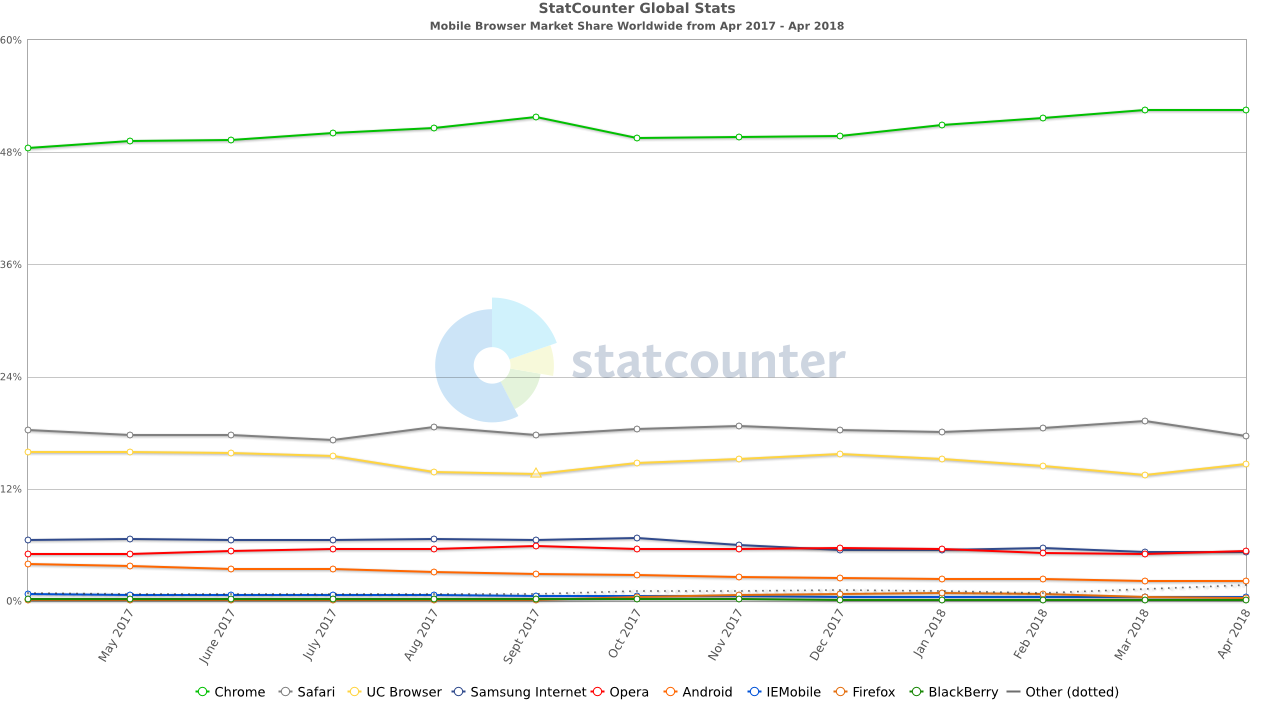
\includegraphics[width=\textwidth]{images/browsers-stats.png}
    
\end{frame}

\begin{frame}

    \frametitle{Datos sobre los navegadores}
    \centering
    \large{Los navegadores libres representan menos del 2.5\% del mercado}    
\end{frame}

\begin{frame}

    \frametitle{Los navegadores en iOS...}
    \centering
    
\includegraphics[height=0.7\textheight]{images/browser-meme.png}
    
\end{frame}

\begin{frame}

    \frametitle{Mensajería - Telegram}

    \begin{columns}[c]
        \column{.3\textwidth}
            \begin{center}
                
\includegraphics[height=0.15\textheight]{images/telegram-logo.png}
                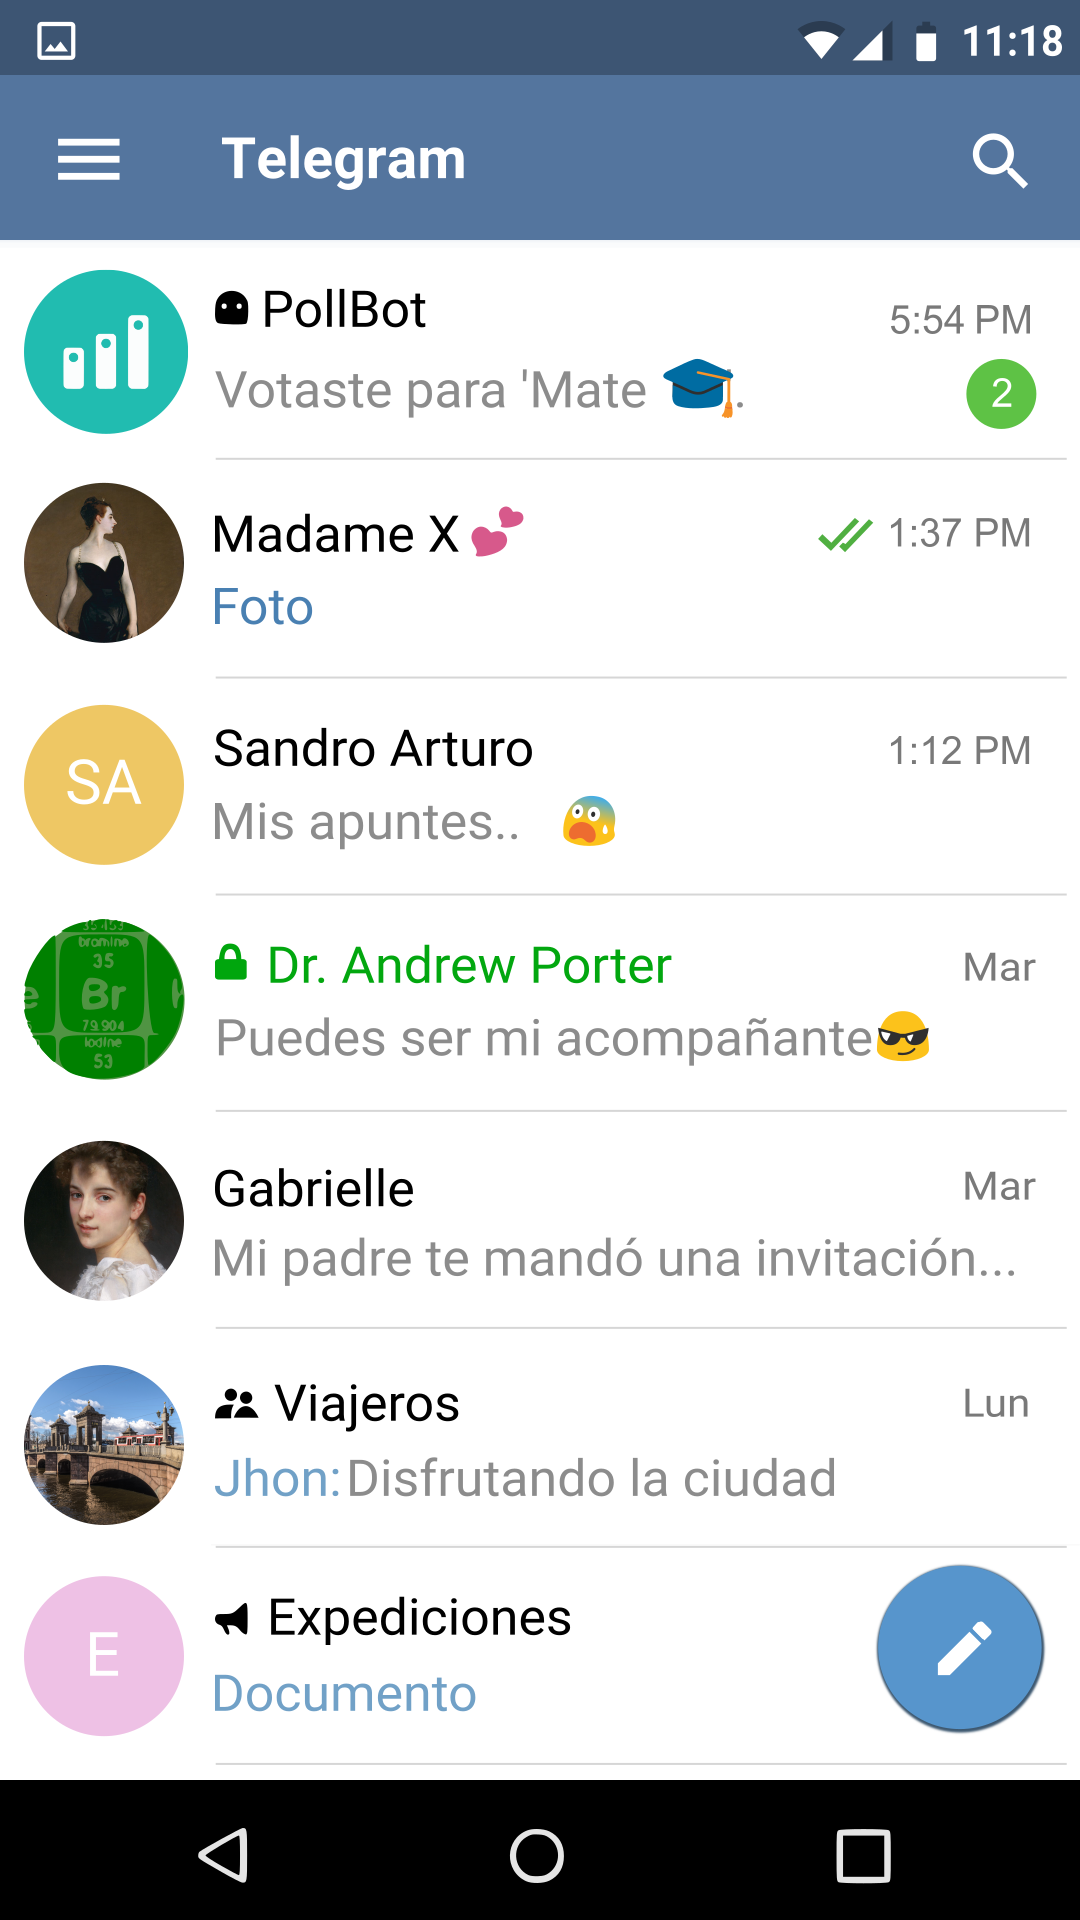
\includegraphics[height=0.5\textheight]{images/telegram-screencap.png}
            \end{center}
        \column{.7\textwidth}
            \begin{itemize}
                \item Plataformas soportadas: Android, iOS
                \item Disponibilidad: Play Store, App Store, F-Droid
                \item Licencia(s): GPLv2 y GPLv3 (clientes), propietaria (servidores)
            \end{itemize}
    \end{columns}

\end{frame}

\begin{frame}

    \frametitle{Mensajería - Telegram}

    \begin{columns}[c]
        \column{.3\textwidth}
            \begin{center}
                
\includegraphics[height=0.15\textheight]{images/telegram-logo.png}
                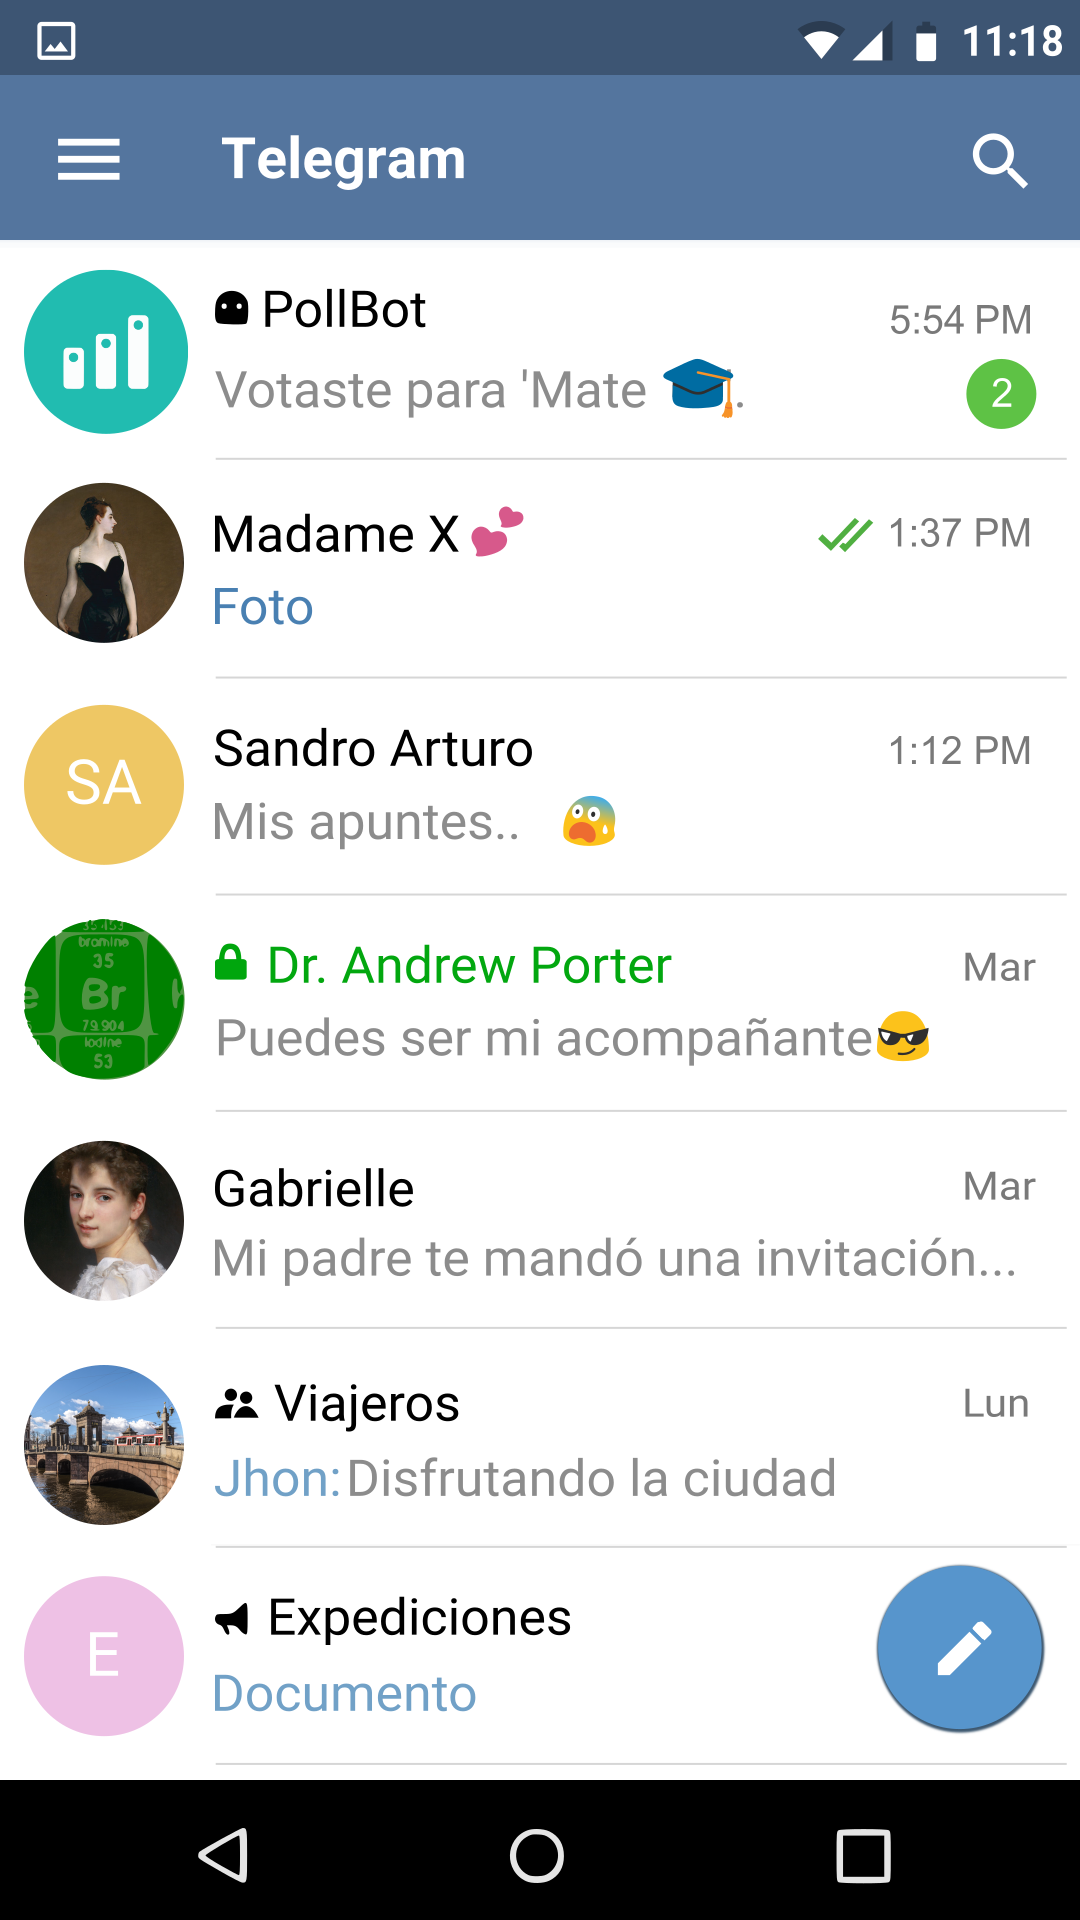
\includegraphics[height=0.5\textheight]{images/telegram-screencap.png}
            \end{center}
        \column{.7\textwidth}
            \begin{itemize}
                \item Plataformas soportadas: Android, iOS
                \item Disponibilidad: Play Store, App Store, F-Droid
                \item Licencia(s): GPLv2 y GPLv3 (clientes), {\color{red}\textbf{\underline{propietaria (servidores)}}}
            \end{itemize}
    \end{columns}

\end{frame}

\begin{frame}

    \frametitle{Mensajería - Wire}

    \begin{columns}[c]
        \column{.3\textwidth}
            \begin{center}
                
\includegraphics[height=0.15\textheight]{images/wire-logo.png}
                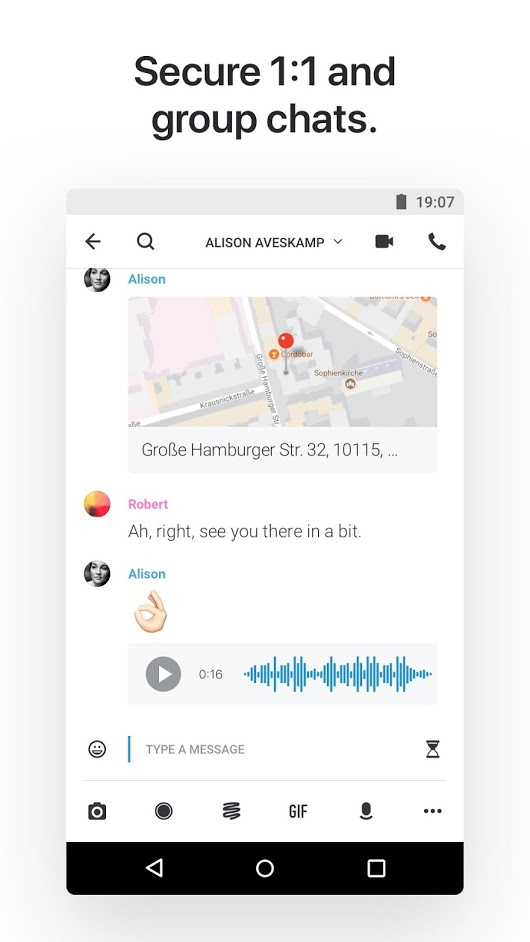
\includegraphics[height=0.5\textheight]{images/wire-screencap.jpg}
            \end{center}
        \column{.7\textwidth}
            \begin{itemize}
                \item Plataformas soportadas: Android, iOS
                \item Disponibilidad: Play Store, App Store
                \item Licencia(s): GPLv3 (clientes), AGPLv3 (servidores)
            \end{itemize}
    \end{columns}

\end{frame}

\begin{frame}
    
    \frametitle{Uso de las aplicaciones de mensajería}
    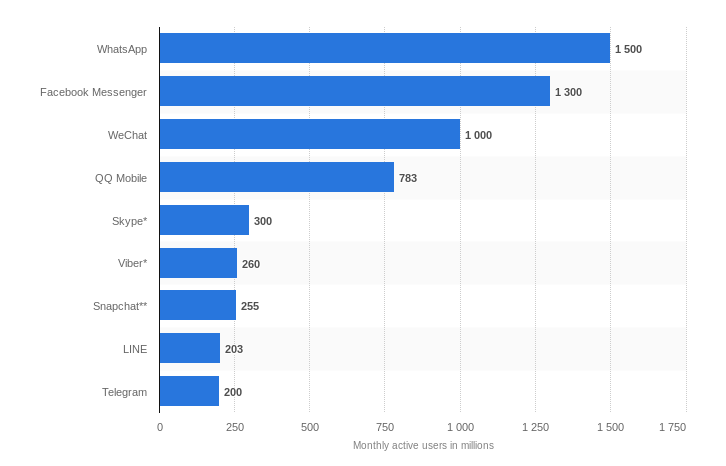
\includegraphics[width=\textwidth]{images/messaging-chart.png}
    \vfill
    \tiny{Datos de Abril de 2018}

\end{frame}

\begin{frame}
    \centering
    \large{De entre las aplicaciones de mensajería más usadas, las libres únicamente son usadas activamente por 200 millones de usuarios. \\ \textbf{Eso es menos del 3.5\% de los usuarios.}}
\end{frame}

\begin{frame}

    \frametitle{Mapas - MAPS.ME}

    \begin{columns}[c]
        \column{.3\textwidth}
            \begin{center}
                
\includegraphics[height=0.15\textheight]{images/mapsme-logo.png}
                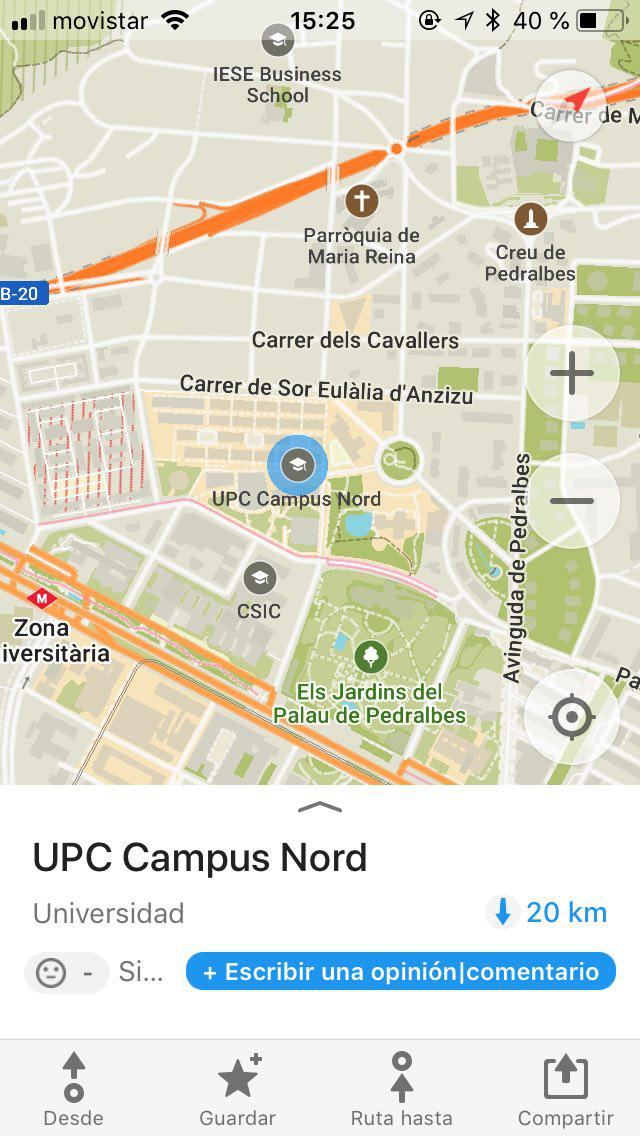
\includegraphics[height=0.5\textheight]{images/mapsme-screencap.jpg}
            \end{center}
        \column{.7\textwidth}
            \begin{itemize}
                \item Plataformas soportadas: Android, iOS
                \item Disponibilidad: Play Store, App Store
                \item Licencia(s): Apache
            \end{itemize}
    \end{columns}

\end{frame}

\begin{frame}

    \frametitle{Email - K9}

    \begin{columns}[c]
        \column{.3\textwidth}
            \begin{center}
                
\includegraphics[height=0.15\textheight]{images/k9-logo.png}
                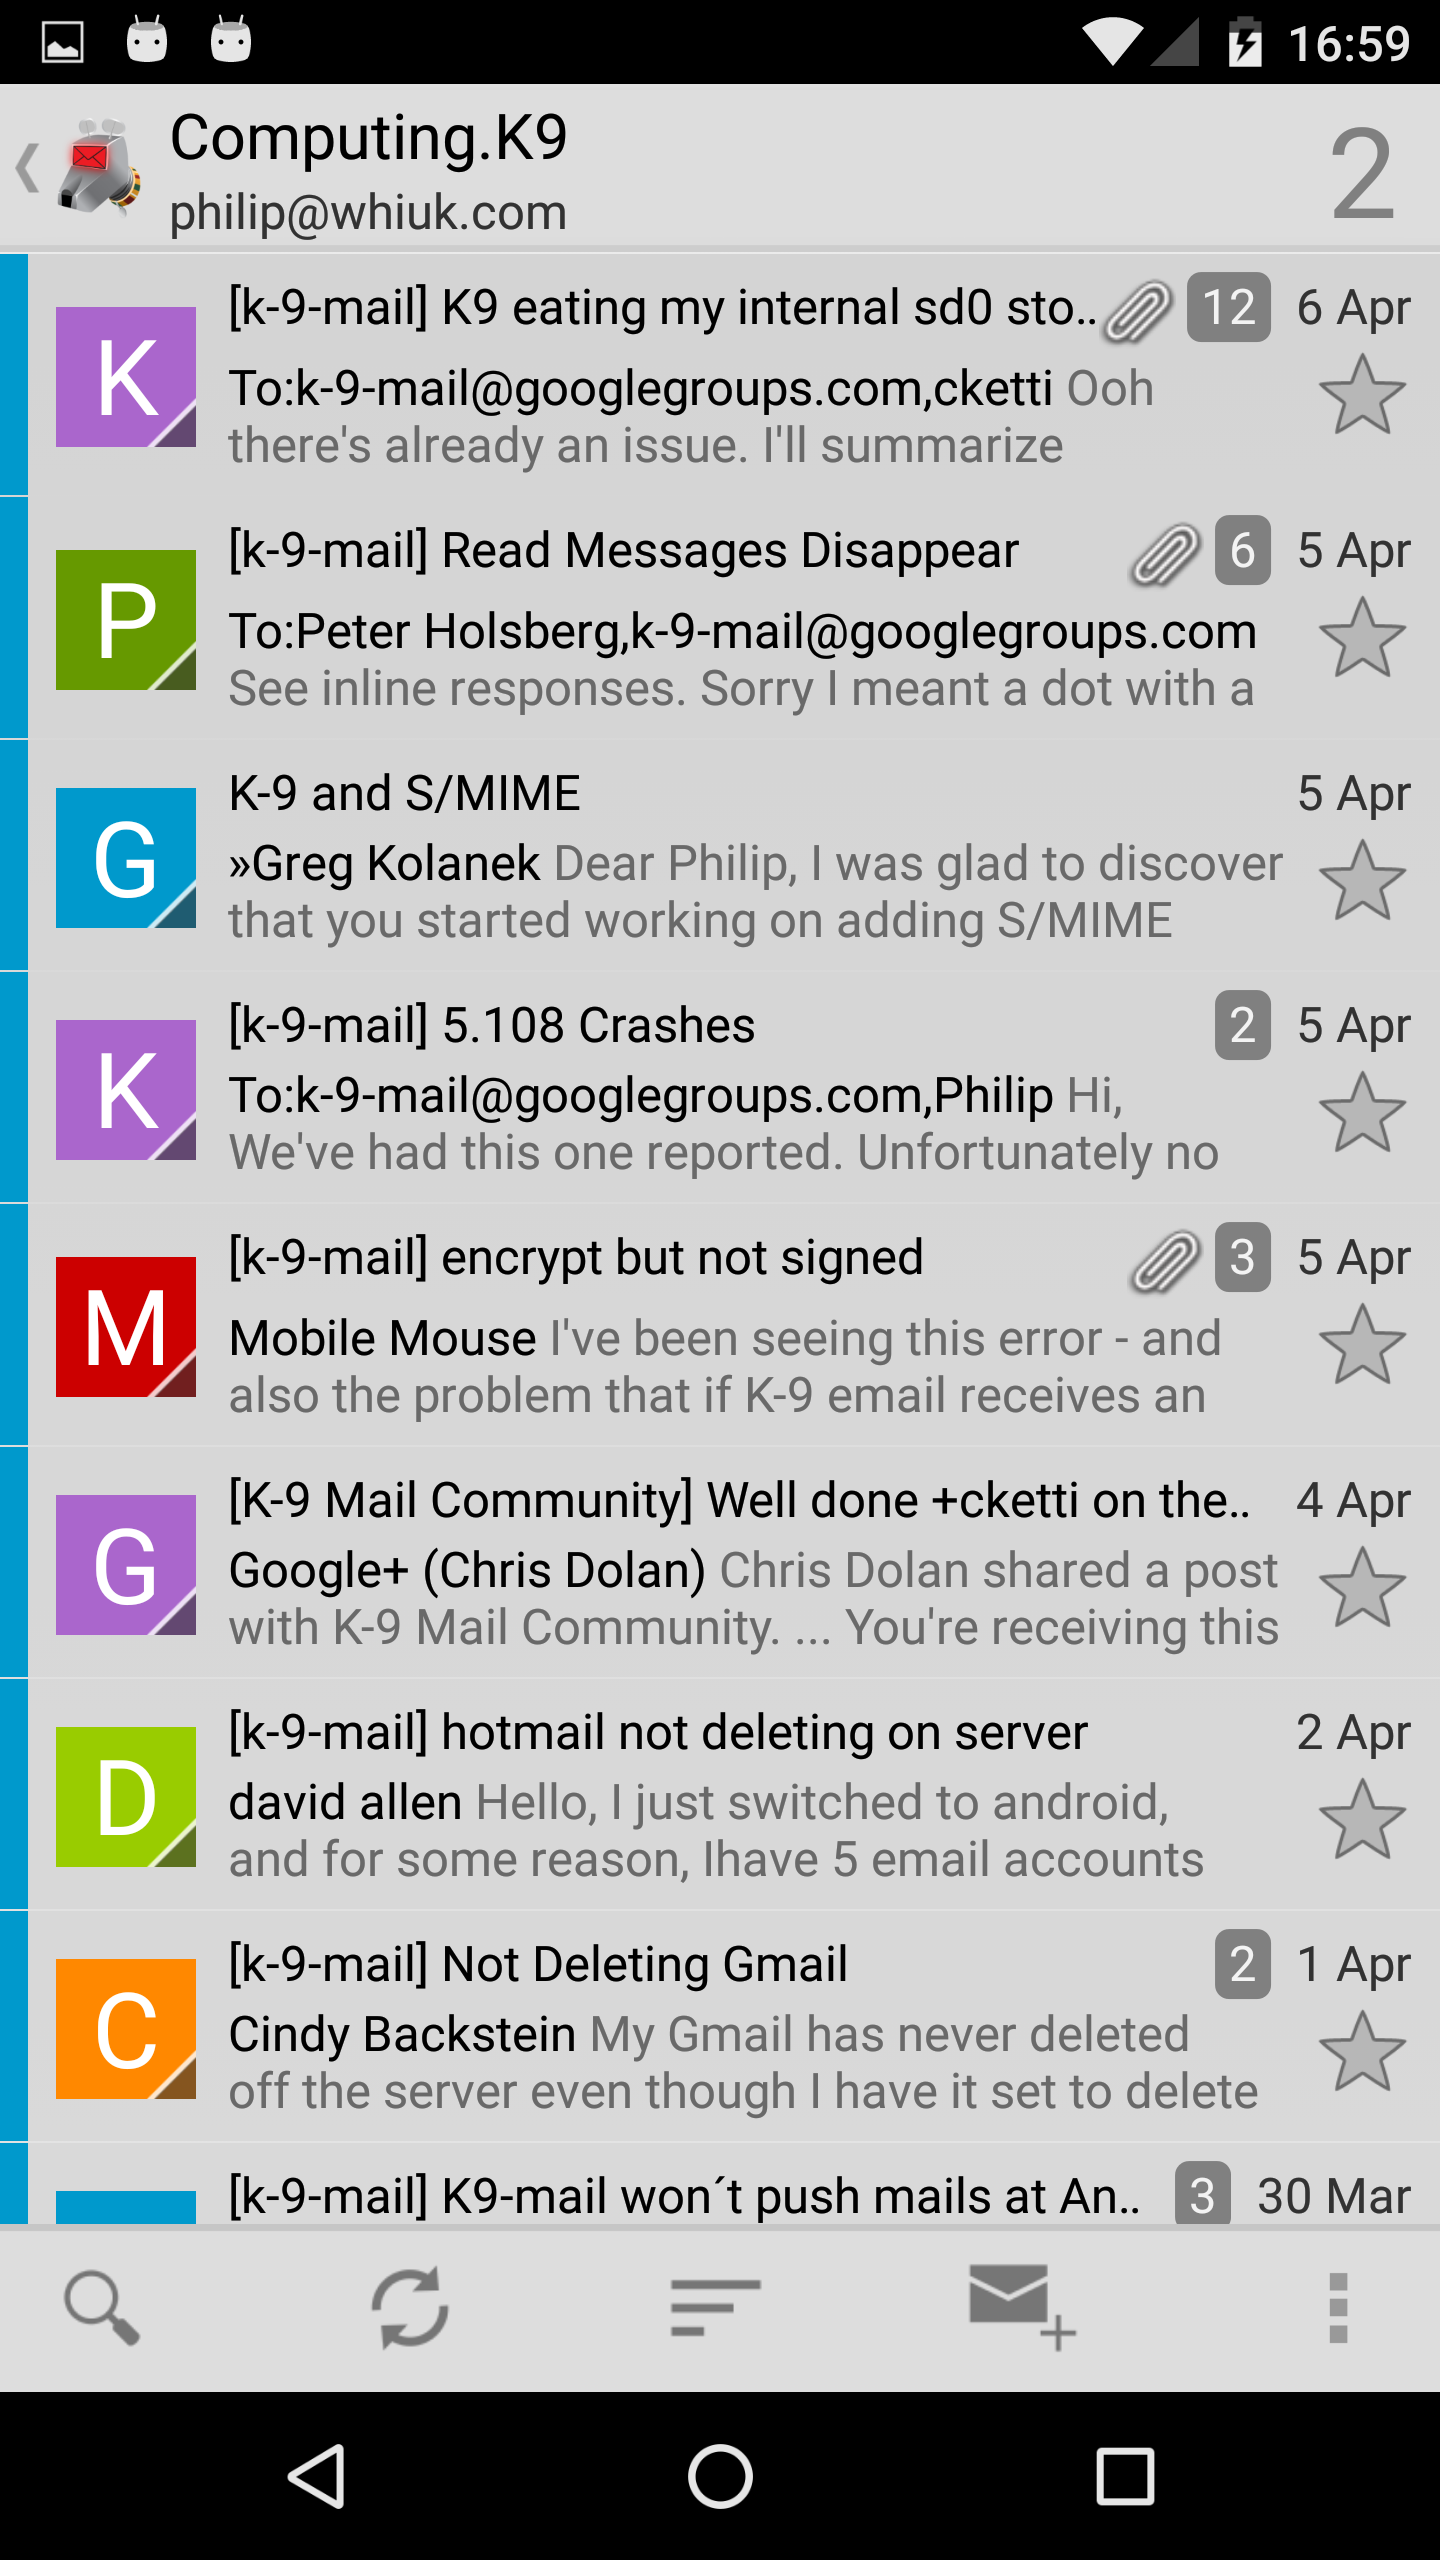
\includegraphics[height=0.5\textheight]{images/k9-screencap.png}
            \end{center}
        \column{.7\textwidth}
            \begin{itemize}
                \item Plataformas soportadas: Android
                \item Disponibilidad: Play Store, F-Droid
                \item Licencia(s): Apache
            \end{itemize}
    \end{columns}

\end{frame}

